% erstewoche/checkliste.tex

In den ersten Wochen an der Uni ist immer viel los: Wir haben euch hier die wichtigsten Punkte zusammengestellt, um die ihr euch in den ersten Tagen bzw. Wochen kümmern solltet. Man findet sich im großen Chaos Universität ziemlich schnell zurecht -- Don't panic!
  
  \begin{enumerate}[label=$\bigcirc$]
  	\item \textbf{Erstwohnsitz in Tübingen anmelden} \\
  		Sofern ihr mit dem Studienbeginn neu nach Tübingen gezogen seid, solltet ihr euch innerhalb von zwei Wochen im Bürgeramt ummelden. Hierfür benötigt ihr die Wohnungsgeberbescheinigung, die ihr beim Einzug von eurem Vermieter bekommt. Es ist ratsam, seinen Erstwohnsitz in Tübingen anzumelden und z.B. das elterliche Wohnhaus als Zweitwohnsitz anzugeben, da Tübingen eine Zweitwohnsitzsteuer erhebt\footnote{Alle Infos der Stadt zum Thema Umzug findet ihr hier \url{https://www.tuebingen.de/12998.html\#/13014}}.
  		%\coronabox{Während der Corona-Pandemie müsst ihr beim Bürgeramt einen Termin vereinbaren. Regelungen dazu und die entsprechenden Telefonnummern findet ihr auf der Webseite\footnote{\url{https://www.tuebingen.de/verwaltung/dienststellen\#buergerbuero\_stadtmitte}}.}
  	
	\item \textbf{Rundfunkbeitrag} \\
		Diesen Brief bekommt ihr normalerweise, sobald ihr euch nach Tübingen umgemeldet habt. Die Rundfunkgebühren müssen nur von einer Person pro Haushalt bezahlt werden, fragt also eure Mitbewohner oder Vermieter, ob schon bezahlt wird! Wenn ihr BaföG bezieht, könnt ihr euch u.U. vom Rundfunkbeitrag befreien lassen. Mehr Infos hierzu auch unter \url{https://www.rundfunkbeitrag.de/}.
  	
  	\item \textbf{Postadresse in ALMA aktualisieren}\\
  		Damit eventuell von der Uni versendete Post auch tatsächlich bei euch ankommt.
  	
  	\item \textbf{WLAN-Zugang mit eduroam einrichten}\\
  		Mit euren ZDV-Login-Daten (i.d.R. \texttt{zxabc12@uni-tuebingen.de} und dem ZDV-Passwort) könnt ihr uniweit kostenlos per WLAN ins Internet. \textbf{Wichtig:} Bindet ein Zertifikat ein! Eine ausführliche Anleitung hierzu findet ihr im Kapitel Infrastruktur.
  	
  	\item \textbf{Mailinglisten anmelden}\\
  	\ifinfo
  		Um wichtige Informationen zum Studium zu bekommen, solltet ihr euch unbedingt auf der info-studium Mailingliste anmelden (mehr dazu im Abschnitt \textit{Mailinglisten}). Dies ist der offizielle Kanal, den die Profs nutzen, um mit euch in Kontakt zu treten.
  	\else
  		Als Kognis solltet ihr euch unbedingt auf den folgenden drei Mailinglisten anmelden; info-studium (offizieller Kommunikationskanal der Info-Profs), kogwis (offizieller Kommunikationskanal der Kogni-Profs und Studienberatung), und versuche (mehr dazu im Abschnitt \textit{Versuchspersonenstunden}, es gibt außerdem die Facebook-Gruppe \textit{Versuchspersonenbörse Tübingen}). Wie ihr euch auf die Listen anmelden könnt, und weitere Mailinglisten findet ihr im Abschnitt \textit{Mailinglisten}.
  	\fi
  	
	\item \textbf{Zum Übungsbetrieb anmelden} \\
	  	Oft muss man, um zur Klausur einer Veranstaltung zugelassen zu werden, eine bestimmte Anzahl an Punkten in den Übungsblättern erreichen. Damit ihr die Übungen machen könnt, müsst ihr euch in der Veranstaltung dazu anmelden. Wie das geht, erfahrt ihr in den ersten Vorlesungen (oft sogar direkt in der ersten Vorlesung, also nicht verpassen!).
	  	
  	\item \textbf{Übungspartner suchen} \\
	  	Übungsblätter im Alleingang zu machen ist zwar möglich, aber schwierig. Sucht euch daher am besten gleich am Anfang pro Veranstaltung mit Übungsbetrieb einen Übungspartner, mit dem ihr die Blätter abgeben könnt.
	  	
	\item \textbf{Bescheinigung für Semesterticket} \\	
		Falls ihr ein Semesterticket erwerben wollt, benötigt ihr dafür eine entsprechende Bescheinigung, die ihr in ALMA unter Studienservice findet. Wo ihr das Semesterticket (auch online) kaufen könnt und weitere Infos sind auf der Webseite der Uni zusammengefasst \url{https://uni-tuebingen.de/de/958}.
	
	\item \textbf{FAQ} \\
	\ifinfo
		Eine Übersicht der häufigsten Fragen und deren Antworten findet ihr hier:
		\link{https://uni-tuebingen.de/de/143913}{FAQ des Fachbereichs}
	\else
		\link{https://uni-tuebingen.de/de/79193}{Eine Übersicht der häufigsten Fragen \\und deren Antworten findet ihr hier}
	\fi
	
  \end{enumerate}

\vfill

\begin{center}
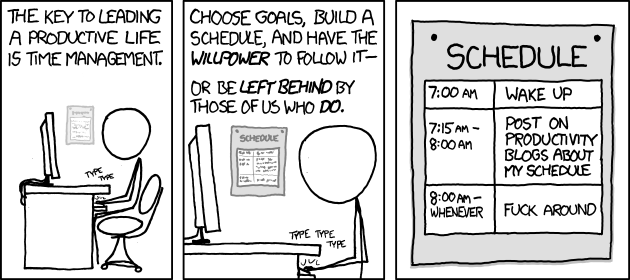
\includegraphics[width=0.8\hsize]{shared/xkcd/time_management.png}
\end{center}
